\chapter{Case study - generating random system properties}

One of the uses of random \gls{FOL} can be to generate random formula that represent system properties. That formula can be used as input for benchmark.

\section{Properties of computer systems}

System properties were first discussed in context of concurrency \cite{Lampert77} as a tool for formal verification multiprocess programs. One of first proposed properties were safety and liveness. These properties can apply to computer systems in general and be expressed in different formal systems.

\textbf{Liveness} \cite{Klimek99} is system property, that states, that something good will eventually happen.
Liveness formula guarantees that there is at least one case, where formula evaluates to true.

\textbf{Safety} \cite{Klimek99} is system property, that states, that something bad will never happens.
Safety formula must always be satisfied.

\subsection{Safety and liveness representation in logic systems}

In \gls{FOL} liveness and safety can be expressed as quantifiers, safety as universal quantifier and liveness as existential quantifier. Every \gls{FOL} can be converted to \gls{CNF}, so system properties can be also represented in \gls{CNF}, if needed. It can be done for example with otter algorithm \cite{McC-Otter-URL} or skolemisation.

In \gls{FOL} system properties could look like:
\begin{itemize}
  \item Safety formula: $\forall_x \neg p(x)$
  \item Safety formula: $\forall_{x,y} \neg p(x,f(y))$ 
  \item Liveness formula: $\exists_x p(x) \lor p1(x)$
  \item Liveness formula: $\exists_{x,y} p(x,f(y))$ 
\end{itemize}

The combinations of quantifiers (that correspond to combinations of liveness and safety properties) are not discussed in this thesis. For example: $\forall_x \exists_y p(x, y)$, $\exists_y \forall_x p(x, y)$.

\subsection{Example}

Example: collisionless lights on crossroad

\noindent
Problem: cars want to drive through crossroad.

\noindent
Safety property: only one light can be green.

\noindent
Liveness property: every light should eventually turn green.

\section{Generating dataset}

Liveness and safety can be expressed as quantifiers those can be converted to CNF. In this section generation of small and big dataset will be presented.
The following code snippet would generate random \gls{FOL} formula, that can represent liveness and safety properties.

\begin{minted}{python}
import math

import src.ast.first_order_logic as fol
from src.ast.exporters.tptp import TPTPExporter
from src.generators import IntegerRange
from src.generators.presets.first_order_logic import CNFFormulaGenerator

if __name__ == '__main__':
    gen = CNFFormulaGenerator(
        functor_names={'f1'}, functor_arity={0}, functor_recursion_depth=0,
        predicate_names={'p1', 'p2'}, predicate_arities={0, 1},
        atom_connectives={''},
        clause_lengths={1, 2, 3},
        variable_names={'V1', 'V2'},
        number_of_clauses=IntegerRange(min=3, max=3),
        number_of_literals=IntegerRange(min=9, max=math.inf)
    ).generate()

    exporter = TPTPExporter(
        output_dir='./temp-out',
        filename_handle=lambda stat: 'generated_cnf_formula'
    )

    for i, formula in enumerate(gen):
        exporter.export(expression=formula, filename_suffix=str(i))
\end{minted}

According to chapter \ref{chap:LogicInternalRepresentation}, \mintinline{python}{CNFFormulaGenerator} is going to generate number of signatures:
\begin{itemize}
  \item 1 variable signature (see table \ref{tab:signatureComparison}): \tptpcodeinline{[V]}
  \item $f(n_{max}, a_{fmin}, a_{fmax}) = f(0, 0, 0) = \sum_{i=0}^{0} \sum_{j=0}^0 f(i, j) = 1$ functor signature \ref{eq:functor}: \tptpcodeinline{[f]}
  \item $p(a_{pmin}, a_{pmax}) = p(0, 1) = \sum_{i=0}^1 p(i) = 3$ predicate signatures \ref{eq:predicate}: \tptpcodeinline{[p, p(V), p(f)]}
  \item $A(connnective) = A(\emptyset) = p(a_{pmin}, a_{pmax}) = 3$ atom signatures \ref{eq:atom}: \tptpcodeinline{[p(V), p(f), p]}
  % \item $L = A(AllowedConnectives) * 2 = 3 * 2 = 6$ literal connectives
  \item $C(l) = \sum_{i=l_{min}}^{i=l_{max}} C(i) = \sum_{i=1}^{3} C(i) = C(1) + C(2) + C(3) = \binom{4 + 1 -1}{1} + \binom{4 + 2 - 1}{2} + \binom{4 + 3 - 1}{3} = 4 + 10 + 20 = 34$ clause signatures \ref{eq:clause}:
    \tptpcodeinline{todo}
\end{itemize}

The exact number of literals and clauses in generated formula is computed internally by Z3 solver. In this case formula must have 3 clauses with length 3.
There are $C(3) = \binom{4 + 3 - 1}{3} = 20$ clause signatures with lenght 3:

\begin{listing}[H]
  \caption{All possible clause signatures with length 3 (random order)}
\begin{tptpcode}
{cnf(name,axiom,p(f)|p|p(V))., cnf(name,axiom,p(V)|p(V)|p(V)).,
 cnf(name,axiom,p(f)|p(f)|p(V))., cnf(name,axiom,p(V)|p|p).,
 cnf(name,axiom,p(V)|p|p(V))., cnf(name,axiom,p(f)|p(V)|p(f)).,
 cnf(name,axiom,p(V)|p(f)|p)., cnf(name,axiom,p(f)|p(f)|p(f)).,
 cnf(name,axiom,p|p(f)|p(f))., cnf(name,axiom,p|p|p(f)).,
 cnf(name,axiom,p|p|p)., cnf(name,axiom,p|p(f)|p).,
 cnf(name,axiom,p(f)|p|p)., cnf(name,axiom,p(V)|p(f)|p(f)).,
 cnf(name,axiom,p|p|p(V))., cnf(name,axiom,p(f)|p|p(f)).,
 cnf(name,axiom,p(V)|p(V)|p(f))., cnf(name,axiom,p(f)|p(f)|p).,
 cnf(name,axiom,p|p(V)|p(V))., cnf(name,axiom,p|p(V)|p(f)).}
\end{tptpcode}
\end{listing}

Based on above signatures, $F_{cnf}(x) = C(l)^x = 20^3 = 8000$ \gls{CNF} formula signatures \ref{eq:cnfformula} can be generated. The final step is post processing (give elements random names and optionally negation sign).

For the benchmark test we shall generate bigger formulas.
100 random formulas were generated from this setup and were benchamarked agains solvers Prover9 and SPASS.

\begin{minted}{python}
    gen = CNFFormulaGenerator(
        functor_names={f'f{i}' for i in range(5)},
        functor_arity={i for i in range(10)}, functor_recursion_depth=0,
        predicate_names={f'p{i}' for i in range(10)}, predicate_arities={i for i in range(10)},
        atom_connectives={''},
        clause_lengths={i for i in range(7, 10)},
        variable_names={f'V{i}' for i in range(10)},
        number_of_clauses=IntegerRange(min=800, max=1000),
        number_of_literals=IntegerRange(min=1000, max=math.inf)
    ).generate(
\end{minted}

\begin{listing}[H]
  \caption{Example of generated formula (limited)}
\begin{tptpcode}
% ----------------------------------------------------------------------------
% File      : 0.p 
% Syntax    : Number of clauses     :  800 (752 non-Horn;   0 unit;   - RR)
%             Number of atoms       : 5602 (  0 equality)
%             Maximal clause size   :    9 (  7 average)
%             Number of predicates  :   10 (2785 propositional; 0-9 arity)
%             Number of functors    :   10 (783 constant; 0-9 arity)
%             Number of variables   :38937 (778 singleton)
%             Maximal term depth    :    0 (  - average)
% 
% ----------------------------------------------------------------------------
cnf(name,axiom,~p4(V5, V8, f8(V2), f4(V9, V7, V6, V1, V8), V2)|p4(V5, V8, f8(V2), f4(V9, V7, V6, V1, V8), V2)|p6(f0(V3, V1, V9, V8, V8, V2, V8, V1, V9), f2(V1, V2, V3, V4, V9, V9, V3), f6(V7, V2, V2))|p4(V5, V8, f8(V2), f4(V9, V7, V6, V1, V8), V2)|p4(V5, V8, f8(V2), f4(V9, V7, V6, V1, V8), V2)|~p6(f0(V3, V1, V9, V8, V8, V2, V8, V1, V9), f2(V1, V2, V3, V4, V9, V9, V3), f6(V7, V2, V2))|p4(V5, V8, f8(V2), f4(V9, V7, V6, V1, V8), V2)|p6(V2, f2(V1, V2, V3, V4, V9, V9, V3), f6(V7, V2, V2))|~p4(V5, V8, f8(V2), f4(V9, V7, V6, V1, V8), V2)).
...
\end{tptpcode}
\end{listing}

All of formulas were UNSAT. The reason may be low number of available names in comparison to number of clauses.

\begin{figure}[ht]
\begin{centering}
  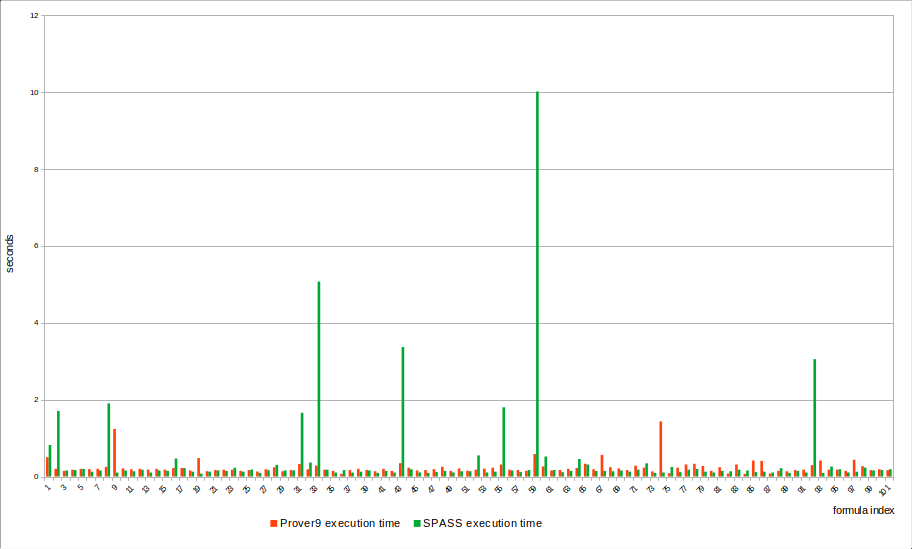
\includegraphics[width=\textwidth]{logic-formula-generator/dataset_analysis/execution_times.png}
  \caption{SPASS and Prover9 execution times on 100 random formulas. All of formulas were UNSAT}
\end{centering}
\end{figure}

